\section{Definizioni fondamentali e primi risultati} \label{sec:def}

\subsection{Sorgenti}
In generale si dice sorgente $S$ un oggetto che emette\footnote{In questi appunti spesso si user\`a lo stesso simbolo sia per la sorgente che per l'alfabeto, anche se ci sono testi in cui si fa differenza, come in \href{http://www.inference.org.uk/mackay/itprnn/book.html}{Information Theory, Inference, and Learning Algorithms}.} simboli $x$ appartenenti ad un alfabeto $X$. La sorgente è nota quando conosciamo la probabilità con cui viene emesso ciascun simbolo. Possiamo distinguere tra:
\begin{itemize}
    \item Sorgenti \textbf{discrete}, in cui l'alfabeto \`e un insieme finito.
    \item Sorgenti \textbf{continue}, in cui l'alfabeto \`e un insieme di simboli infinito numerabile.
\end{itemize}

Sappiamo, comunque, che qualsiasi sorgente continua può essere trasformata in una sorgente numerica (in
particolare digitale) grazie alle operazioni di campionamento e quantizzazione. Le sorgenti con cui abbiamo a che fare nei moderni sistemi informativi sono infatti sostanzialmente sempre sorgenti discrete. Per questo motivo la nostra attenzione sarà principalmente rivolta alle sorgenti discrete anche se poi i risultati verranno generalizzati al caso continuo perché ci sono contesti (in particolare il canale di comunicazione) in cui abbiamo a che fare con segnali/sorgenti continui. \\
I simboli emessi dalla sorgente sono delle \hyperref[sec:prob]{\textbf{variabili aleatorie}} (altrimenti \textit{non ci sarebbe informazione da
trasmettere}) e quindi ci si riferisce sempre a variabili e processi aleatori. Quando, infatti, si considera l’emissione successiva di simboli nel tempo si ha un \hyperref[sec:stoc]{\textbf{processo stocastico}}, ovvero una sequenza di variabili aleatorie indicizzate nel tempo.

Un'altra distinzione che possiamo fare nelle sorgenti dipende dal legame tra simboli successivi (emessi ad istanti successivi dalla sorgente). Se questi sono dipendenti gli uni dagli altri la sorgente si dice \textbf{con memoria}, altrimenti si dice \textbf{senza memoria} e le variabili aleatorie sono indipendenti e identicamente distribuite. \\
Le sorgenti senza memoria sono più semplici ma più rare. Un lancio di monete è una sorgente senza memoria: in questo caso basta conoscere la probabilità di ogni singolo simbolo perché la probabilità congiunta è il prodotto delle singole probabilità. Le sorgenti con memoria invece sono più complesse ma sono anche quelle che di solito si trovano in pratica, e sono caratterizzate dalle probabilità congiunte. Ad esempio un testo scritto: ci sono ovviamente dei legami tra le lettere che escono, ad esempio una $q$ è seguita da una $u$, perché devono rispettare una sintassi. 
\subsection{Informazione ed Entropia}
Prima di tutto il problema della teoria dell’informazione è definire, rappresentare matematicamente e
quantificare l’informazione che viene prodotta da una sorgente. L’informazione può essere di tipo:
\begin{itemize}
    \item \textbf{Semantico}, ovvero riguardare il significato del messaggio.
    \item \textbf{Sintattico}, ovvero riguardare i simboli che si usano e come questi sono relazionati tra loro - come \`e costruito il messaggio.
\end{itemize}
La teoria dell’informazione si occupa \textit{solo dell’aspetto \textbf{sintattico}} (o simbolico): a livello di sistema di comunicazione non ci interessa la semantica, ovvero cosa significa un dato messaggio (dal momento che incontriamo il problema della soggettività dell’informazione) ma la \textit{quantità} di informazione che questo porta.\\ 
Shannon sviluppò l’idea di definire l’informazione legata ad un evento $x$ solo in relazione
alla probabilità $p(x)$ che quell’evento avvenga, in particolare ebbe l'intuizione di imporre che il contenuto informativo dell'evento fosse tanto maggiore quanto pi\`u bassa fosse la probabilit\`a dell'evento associato. Le propriet\`a che la definizione di informazione $I(\cdot)$ deve soddisfare sono:
\begin{itemize}
    \item Deve essere una funzione (continua) della probabilit\`a: $I(x) = f(p(x))$ e deve essere $f(p(x)) \in (0,1]$ (un evento che non pu\`o avvenire non \`e di interesse). 
    \item Deve essere $I(1) = 0$, dal momento che un evento certo non porta informazione.
    \item Deve essere $p(x) \to 0^+ \implies I(x) \to \infty$, ovvero che un evento raro porti molta informazione, e quindi che la funzione $f$ sia decrescente.
\end{itemize}

Sia $S$ una sorgente (una variabile aleatoria discreta) che emette simboli su un alfabeto $X=\{x_1, x_2, \dots, x_M\}$ con una distribuzione $p(x) = Pr\{S=x\}, x\in X$.
\defn{\textit{Informazione}}: L'informazione associata al simbolo $x$ \`e definita\footnote{Il logaritmo si intende implicitamente in base 2 anche se pu\`o essere ovviamente operato un cambio di base: $\log_b p = \log_b a \log_a p$. In questo caso cambia solamente l'unit\`a con cui si misura l'informazione. Per $b=2$ si ha il $bit$, per $b=3$ il $trit$, per $b=e$ il $neper$ e cos\`i via. Si veda la Figura \ref{fig:autoinf}b per l'andamento della funzione di informazione al variare della base $b$.} come 
\begin{equation}
I(x) \coloneqq \log \frac{1}{p(x)}
\end{equation}
Se si hanno più eventi \textit{indipendenti}, essendo la probabilità congiunta degli eventi il prodotto delle probabilità, l’informazione complessiva è la somma delle singole informazioni:
\begin{equation}
I(x, y) = \log \frac{1}{p(x,y)} = \log \frac{1}{p(x)p(y)} = \log \frac{1}{p(x)} + \log \frac{1}{p(y)} = I(x) + I(y)
\end{equation}
\textit{\`E importante sottolineare come l’informazione sia solo legata alla probabilità  che un evento accada, non è in alcun modo legata alla natura dell'evento}. \\
Se consideriamo una sorgente $S$ discreta senza memoria (DMS): si ha che l'informazione media della sorgente \`e data dal valore atteso dell'informazione:

\defn{\textit{Entropia}}: L'entropia associata alla sorgente DMS \`e definita come
\begin{equation}
H(S) \coloneqq \mathbb{E}_p [I(x)] =  \sum_{x \in X} p(x) \info{x} = - \sum_{x \in X} p(x) \log p(x)
\end{equation}
e si misura in \textit{bit/simbolo}. Vedremo pi\`u avanti come l’entropia dia una misura del “costo minimo” per rappresentare un’informazione, ovvero il \textit{minimo numero medio di bit che servono per rappresentare le informazioni inviate da una sorgente}. \\
Quando si ha $p(x)=0$ si adotta la convenzione $0 \times \info{0} \coloneqq 0$ dal momento che 
\begin{equation}
\lim_{x\to0^+} x \log \frac{1}{x} = 0
\end{equation}

\begin{figure}[!tbp]
  \centering
  \subfloat{\includegraphics[width=0.5\textwidth]{img/sorgente.jpg}\label{fig:sorge}}
  \hspace{15pt}
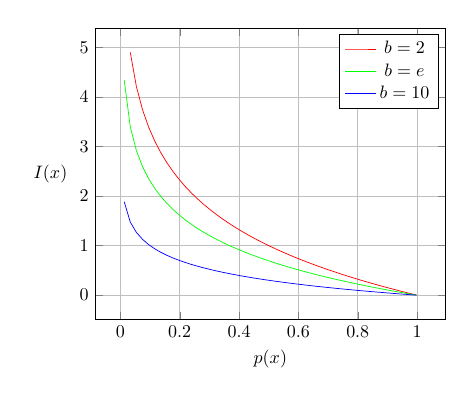
\begin{tikzpicture}[thick,scale=0.65]
\begin{axis}[domain=-.5:20, samples=1000,grid=major,
    restrict y to domain=0:5,xlabel=$p(x)$,ylabel=$I(x)$, ylabel style={rotate=-90},]
          \addplot [color=red]    {-log2(x)};
\addplot [color=green]  {-log2(x)/log2(e)};
\addplot [color=blue] {-log2(x)/log2(10)}; 
\legend{$b=2$, $b=e$, $b=10$}
\end{axis}
\end{tikzpicture}
  \caption{Rappresentazione schematica di una sorgente e grafico della funzione di informazione.}
  \label{fig:autoinf}
\end{figure}

\begin{mybox}{green}{\textit{\textbf{Esempio 1} : \textbf{Sorgente Binaria}}}
Consideriamo una sorgente $S$ che emette due soli simboli: $X = \{x,y\}$ con probabilit\`a $p(x) = q$ e $p(y) = 1- q$. Si ha che 
\begin{equation}
H(S) = H(q) = q \log \frac{1}{q} + (1-q)\log \frac{1}{1-q}
\end{equation}
Ad esempio se $q=0.7$ si avrebbe $H(q) \approx 0.88$ $bit/simbolo$. Quand'\`e che l'entropia di una sorgente binaria \`e massima? Si vede facilmente che il massimo si ottiene in:
\begin{align*}
    &\frac{d}{dq} H(q) = \frac{d}{dq} \Big \{ -q \log q - (1-q) \log{1-q} \Big \} = \\
    &= - \Big \{ \log q + q \frac{1}{q} \log e -\log(1-q) - (1-q)\frac{1}{1-q} \log e \Big \} = \\
    &= \log{(1-q)} - \log{q} = 0 
\end{align*}
ovvero quando si ha
\[
1-q = q \implies q = \frac{1}{2}
\]
Quindi si ha che l'entropia di una sorgente binaria \`e massima quando i due simboli sono equiprobabili e vale $H(q) = 1$.

\begin{figure}[H]
    \centering
    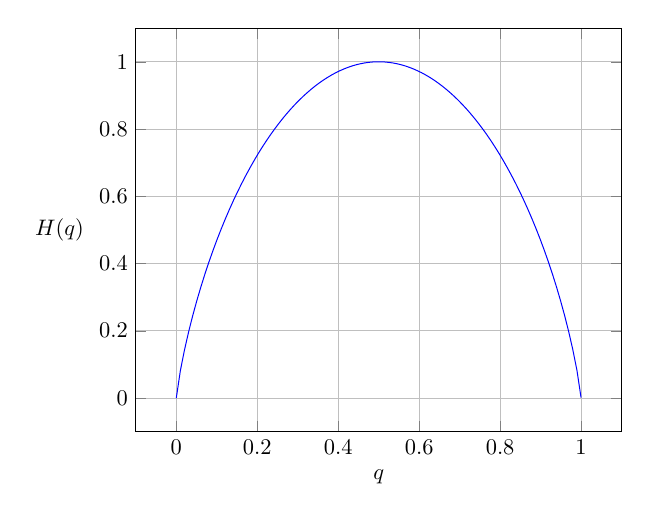
\begin{tikzpicture}[thick,scale=0.9, every node/.style={scale=0.9}]
\begin{axis}[domain=0:1, samples=100,grid=major,
    restrict y to domain=0:1,xlabel=$q$,ylabel=$H(q)$, ylabel style={rotate=-90},]
          \addplot [color=blue]    {-x*log2(x) - (1-x)*log2(1-x)};
\end{axis}
\end{tikzpicture}
    \caption{Entropia di una sorgente binaria, al variare di $q$.}
    \label{fig:binentropy}
\end{figure}
\end{mybox}

Si hanno poi queste due propriet\`a, in cui la seconda \`e una generalizzazione di quanto appena visto per una sorgente binaria:
\begin{enumerate}
    \item $H(S) \geq 0$ dal momento che $0 \leq p(x) \leq 1 \implies \info{x} \geq 0$. 
    \item $H(S) \leq \log M$ con $H(S) = \log M \iff$ i simboli sono equiprobabili.
\end{enumerate}
Vediamo la dimostrazione per questa seconda propriet\`a: 
\begin{tcolorbox}[enhanced, breakable, frame hidden]
\textbf{Dim}: Vogliamo provare che $H(S) - \log M \leq 0$. Si ha che
\begin{align*}
&H(S) - \log M = \\
&= \sum_{x \in X} p(x) \info{x} - \log M \overset{\alpha}{=} \\
&= \sum_{x \in X} p(x) \info{x} - \sum_{x \in X} p(x) \log M = \\
&= \sum_{x \in X} p(x) \Big ( \log \frac{1}{Mp(x)} \Big ) = \\
&= \log{e} \bigg [ \sum_{x \in X} p(x) \Big ( \ln \frac{1}{Mp(x)} \Big ) \bigg ] \overset{\beta}{\leq} \\
&\leq \log{e} \bigg [ \sum_{x \in X} p(x) \Big ( \frac{1}{Mp(x)} - 1 \Big ) \bigg ] = \\
&= \log{e} \bigg [ \sum_{x \in X} \Big ( \frac{1}{M} - p(x) \Big ) \bigg ] = \\
&= \log{e} \bigg [ 1 - \sum_{x \in X} p(x) \bigg] \overset{\alpha}{=} 0 \\
\end{align*} 
Si ha poi che la disuguaglianza vale con l'uguale quando, $\forall x \in X$:
\[
\ln \frac{1}{Mp(x)} = \frac{1}{Mp(x)} -1 \iff \frac{1}{Mp(x)} = 1 \iff p(x) = \frac{1}{M}
\]
ovvero quando tutti i simboli $x$ sono equiprobabili. $\square$
\end{tcolorbox}
Dette $p,q$ due distribuzioni sullo stesso alfabeto $X$ si definisce una quantit\`a importante: 
\defn{\textit{Entropia Relativa}}: L'entropia relativa, detta anche \textit{divergenza di Kullback-Leibler} è una misura non simmetrica{\footnote{Anche se è spesso pensata come una distanza, la divergenza KL non è una vera e propria metrica - per esempio, infatti, non è simmetrica: la KL da $p$ a $q$ non è in genere la stessa KL da $q$ a $p$. Tuttavia, la sua forma infinitesimale, in particolare la sua matrice Hessiana, è un tensore metrico: \`e l'\href{https://it.wikipedia.org/wiki/Informazione_di_Fisher}{informazione metrica di Fisher}. Oltre a non essere simmetrica non pu\`o essere una distanza dal momento che non vale la disuguaglianza triangolare.}} della differenza tra due distribuzioni di probabilità. Misura infatti l'inefficienza (la perdita di informazione che si ha) nell'assumere che la distribuzione di probabilit\`a sia $q$ quando quella reale \`e $p$.
\begin{equation}
D(p\|q) \coloneqq \sum_{x \in X} p(x) \log \frac{p(x)}{q(x)}
\end{equation}
Anche per l'entropia relativa si pu\`o mostrare un'importante propriet\`a, quella della non-negativit\`a:
\begin{itemize}
    \item $D(p \| q) \geq 0$ con $D(p \| q) = 0 \iff p = q$
\end{itemize}
\begin{tcolorbox}[enhanced, breakable, frame hidden]
\textbf{Dim}: Vogliamo mostrare che $-D(p \| q) \leq 0$. Si ha:
\begin{align*}
    -D(p \| q) = \sum_{x \in X} p(x) \log \frac{q(x)}{p(x)} = \log e \sum_{x \in X} p(x) \ln \frac{q(x)}{p(x)} \overset{\beta}{\leq} \\
    \leq \log e \sum_{x \in X} p(x) \Big ( \frac{q(x)}{p(x)} - 1 \Big ) = \log e \Big ( \sum_{x \in X} q(x) - \sum_{x \in X} p(x) \Big ) = 0 \\
    \square
\end{align*}
\end{tcolorbox}
L'entropia relativa \`e importante in molti ambiti diversi della teoria dell'informazione (e non solo) ed ha una interpretazione legata alla costruzione dei codici: se  abbiamo  una  sorgente $S$ che  emette  simboli con distribuzione $p$ per rappresentarla  possiamo costruire un  codice con lunghezza  $H(p)$ bit/simbolo, se però usiamo un codice costruito per una  distribuzione $q$ c’è bisogno  in media di una lunghezza  $H(p)+D(p\|q)$ per rappresentarla. \\
Data una variabile aleatoria congiunta $(X, Y)$ con distribuzione di probabilit\`a congiunta $p(x,y)$ si definisce l'entropia congiunta delle variabili $X$ e $Y$ come
\defn{\textit{Entropia Congiunta}}: \\ Sia $x \in X = \{x_1, \dots, x_M \}$ e $y \in Y = \{y_1, \dots, y_Q \}$ una coppia di variabili aleatorie con distribuzione congiunta $p(x,y)$. Si ha che l'entropia congiunta tra $X$ e $Y$ \`e definita come:
\begin{equation}
H(X,Y) \coloneqq \sum_{x \in X} \sum_{y \in Y} p(x,y) \log \frac{1}{p(x,y)}
\end{equation}
Una quantit\`a strettamente correlata all'entropia congiunta \`e la:
\defn{\textit{Entropia Condizionata}}: L'entropia condizionata \`e definita come:
\begin{equation}
H(X|Y) = \sum_{x \in X} \sum_{y \in Y} p(x,y) \log \frac{1}{p(x|y)}
\end{equation}
Per quanto riguarda il rapporto tra entropia congiunta e condizionata si pu\`o vedere che:
\begin{equation}
H(X,Y) = H(X) + H(Y|X) = H(Y) + H(X|Y)
\end{equation}
che prende il nome di \textit{chain rule} per l'entropia.
\begin{tcolorbox}[enhanced, breakable, frame hidden]
\textbf{Dim}: Mostriamo che $H(X,Y) = H(X) + H(Y|X)$, vale l'analogo per l'altro caso.
\begin{align*}
    H(X,Y) &= \sum_{x \in X} \sum_{y \in Y} p(x,y) \log \frac{1}{p(x,y)} \overset{\gamma}{=} \sum_{x \in X} \sum_{y \in Y} p(x,y) \log \frac{1}{p(y|x)p(x)} = \\
    &= \sum_{x \in X} \sum_{y \in Y} p(x,y) \Big [ \log \frac{1}{p(x)} + \log \frac{1}{p(y|x)} \Big] = 
\end{align*}
\begin{align*}
    &= \sum_{x \in X} \sum_{y \in Y} p(x,y) \log \frac{1}{p(x)} + \sum_{x \in X} \sum_{y \in Y} p(x,y) \log \frac{1}{p(y|x)} = \\
    &\overset{\delta}{=} \sum_{x \in X} p(x) \info{x} + \sum_{x \in X} \sum_{y \in Y} p(x,y) \log \frac{1}{p(y|x)} = \\
    &= H(X) + H(Y|X) \hspace{200pt} \square
\end{align*}
\end{tcolorbox}
La chain rule per l'entropia pu\`o essere generalizzata a $m$ variabili aleatorie $X_1, X_2, \dots, X_m$:
\begin{equation}
    H(X_1, X_2, \dots, X_m) = H(X_1) + H(X_2|X_1) + H(X_3|X_1, X_2) + \dots + H(X_m|X_1, \dots, X_{m-1})
\end{equation}
ricordando che la chain rule per la probabilit\`a \`e data da:
\begin{equation}
\label{eqn:probchain}
    p(x_1, x_2, \dots, x_m) = p(x_1) \cdot p(x_2|x_1) \cdot p(x_3|x_1, x_2) \cdot \dots \cdot p(x_m|x_1, \dots, x_{m-1})
\end{equation}
Una propriet\`a importante dell'entropia condizionata \`e che, in generale, si ha
\begin{equation}
    H(X|Y) \leq H(X)
\end{equation}
ovvero che il condizionamento non pu\`o far aumentare l'entropia (\textit{information can't hurt}).
\begin{tcolorbox}[enhanced, breakable, frame hidden]
\textbf{Dim}: Mostriamo che $H(X|Y) - H(X) \leq 0$
\begin{align*}
    H(X|Y) - H(X) &= \sum_{x \in X} \sum_{y \in Y} p(x,y) \log \frac{1}{p(x|y)} - \sum_{x \in X} p(x) \info{x} \overset{\delta}{=} \\
    &= \sum_{x \in X} \sum_{y \in Y} p(x,y) \log \frac{1}{p(x|y)} - \sum_{x \in X} \sum_{y \in Y} p(x,y) \info{x} =\\
    &= \sumx \sumy p(x,y) \log \frac{p(x)}{p(x|y)} = \log e \sumx \sumy p(x,y) \ln \frac{p(x)}{p(x|y)} \overset{\beta}{\leq} \\
    &\leq \log e \sumx \sumy p(x,y) \Big [ \frac{p(x)}{p(x|y)} - 1 \Big ] = \log e \sumx \sumy p(x,y) \Big [ \frac{p(x)p(y)}{p(x,y)} - 1 \Big] = \\ 
    &= \log e \bigg [ \sumx p(x) \sumy p(y) - \sumx \sumy p(x,y) \bigg] = 0 \hspace{100pt} \square
\end{align*}
\end{tcolorbox}
Ovviamente vale anche $H(Y|X) \leq H(Y)$ per cui, per l'entropia congiunta, vale anche questa disuguaglianza:
\begin{equation}
\label{eqn:leq}
    H(X,Y) \leq H(X) + H(Y)
\end{equation}

\subsection{Informazione Mutua}
Un'altra grandezza fondamentale \`e l'informazione mutua tra due sorgenti. Questa misura in un certo senso il grado di dipendenza di due variabili aleatorie, ovvero misura \textit{quanta informazione di una variabile aleatoria \`e contenuta nell'altra}. Pu\`o essere pensata come la quantit\`a di riduzione dell'incertezza su una variabile aleatoria quando si osserva l'altra. \`E definita come
\defn{\textit{Informazione mutua:}} Date due variabili aleatorie $X, Y$ si ha che l'informazione mutua \`e definita come:
\begin{equation}
    I(X;Y) \coloneqq \sumx \sumy p(x,y) \log \frac{p(x,y)}{p(x)p(y)}
\end{equation} 
Data questa definizione si vede subito che
\begin{equation}
    I(X;Y) = D \Big ( p(x,y) \| p(x)p(y) \Big )
\end{equation}
ovvero che l'informazione mutua \`e \textit{l'entropia relativa tra la distribuzione congiunta e il prodotto delle marginali}. Da questa considerazione si ha subito una prima propriet\`a per l'informazione mutua:
\begin{equation}
    I(X;Y) \geq 0
\end{equation}
Si ha inoltre che, se le due variabili aleatorie sono indipendenti, $p(x,y) = p(x)p(y)$, si ha $I(X;Y) = 0$ ovvero non c'\`e distanza tra le due distribuzioni. Viceversa più le variabili aleatorie sono tra loro legate più l’informazione mutua cresce, difatti la differenza tra la distribuzione congiunta e il prodotto delle due aumenta. \\
Se $X$ e $Y$ sono indipendenti, allora la conoscenza di $X$ non dà alcuna informazione riguardo a $Y$ e viceversa, perciò la loro mutua informazione è zero. All'altro estremo, se $X$ e $Y$ sono identiche allora tutte le informazioni trasmesse da $X$ sono condivise con $Y$: la conoscenza di $X$ determina il valore di $Y$ e viceversa.\\
L’informazione mutua è strettamente collegata all’entropia, infatti:
\begin{equation}
    I(X;Y) = H(X) - H(X|Y) = H(Y) - H(Y|X)
\end{equation}
\begin{tcolorbox}[enhanced, breakable, frame hidden]
\textbf{Dim}: Mostriamo che $I(X;Y) = H(X) - H(X|Y)$, l'altro caso \`e equivalente.
\begin{align*}
    I(X;Y) &= \sumx \sumy p(x,y) \log \frac{p(x,y)}{p(x)p(y)} = \sumx \sumy p(x,y) \frac{p(x|y)p(y)}{p(x)p(y)} = \\
    &= \sumx \sumy p(x,y) \log \frac{p(x|y)}{p(x)} = \sumx \sumy p(x,y) \Big [ \log \frac{1}{p(x)} - \log \frac{1}{p(x|y)} \Big ] = \\
    &= \sumx \sumy p(x,y) \log \frac{1}{p(x)} - \sumx \sumy p(x,y) \log \frac{1}{p(x|y)} =\\ 
    & = \sumx p(x) \info{x} - \sumx \sumy p(x,y) \log \frac {1}{p(x|y)} = H(X) - H(X|Y) \hspace{30pt} \square
\end{align*}
\end{tcolorbox}
In sostanza quindi l’informazione mutua è una differenza tra entropie: l’entropia di una variabile aleatoria meno l’incertezza di quella variabile aleatoria una volta che ho conosciuto l'altra. Si ha inoltre che
\begin{itemize}
    \item L'informazione mutua \`e simmetrica: $I(X;Y) = I(Y;X)$.
    \item $I(X;Y) = H(X) + H(Y) - H(X,Y)$ (dalla chain rule per l'entropia).
    \item Nel caso discreto vale $I(X;X) = H(X)$ (dal fatto che $H(X|X) = 0$) per cui si ha $I(X;X) \geq I(X;Y)$, ovvero che una variabile $X$ contiene almeno tanta informazione riguardo a sé stessa di quanta ne può fornire una qualsiasi altra variabile $Y$.
\end{itemize}
\begin{figure}[!tbp]
  \centering
  \subfloat{\includegraphics[width=0.4\textwidth]{img/infomut.jpg}\label{fig:f1}}
  \hspace{25pt}
  \subfloat{\includegraphics[scale=0.5]{img/mutinfo.jpg}\label{fig:f2}}
  \caption{Due rappresentazioni equivalenti delle relazioni tra entropia e informazione mutua.}
\end{figure}

\subsection{Estensione di una sorgente}
Siano $X_1, X_2, \dots, X_n$ un numero $n$ di variabili aleatorie identicamente distribuite ($i.d.$) (come ad esempio nella trasimissione di un messaggio in cui ogni simbolo emesso appartiene allo stesso alfabeto). L'entropia congiunta di queste $n$ variabili aleatorie rappresenta una grandezza importante:
\begin{equation}
    H(X_1, X_2, \dots, X_n) = \sum_{x_1 \in X_1} \sum_{x_2 \in X_2} \dots \sum_{x_n \in X_n} p(x_1, x_2, \dots, x_n) \log \frac{1}{p(x_1, x_2, \dots, x_n)}
\end{equation}
\defn{\textit{Estensione della sorgente:}} La quantit\`a $(X_1, X_2, \dots, X_n)$ prende il nome di estensione della sorgente e si indica con $X^n$. Dal momento che queste $n$ variabili aleatorie sono $i.d$ si ha che $H(X) = H(X_1) = H(X_2) = \dots = H(X_n)$. Nel caso in cui non si ha memoria, oveero quando queste $n$ variabili aleatorie sono anche indipendenti (sono quindi $i.i.d$) si ha che
\begin{equation}
    H(X^n) \coloneqq H(X_1, X_2, \dots, X_n) = nH(X)
\end{equation}
\begin{tcolorbox}[enhanced, breakable, frame hidden]
\textbf{Dim}:
\begin{align*}
    &H(X_1, X_2, \dots, X_n) = \sum_{x_1 \in X_1} \sum_{x_2 \in X_2} \dots \sum_{x_n \in X_n} p(x_1, x_2, \dots, x_n) \log \frac{1}{p(x_1, x_2, \dots, x_n)} = \\
    &=\sum_{x_1 \in X_1} \sum_{x_2 \in X_2} \dots \sum_{x_n \in X_n} p(x_1)p(x_2)\dots p(x_n) \log \frac{1}{p(x_1)p(x_2)\dots p(x_n)} = \\
    &=\sum_{x_1 \in X_1} \sum_{x_2 \in X_2} \dots \sum_{x_n \in X_n} p(x_1)p(x_2)\dots p(x_n) \Big [ \info{x_1} + \info{x_2} \dots + \info{x_n} \Big]
\end{align*}
Si ha quindi la somma di $n$ termini. Analizziamo il generico elemento $k$ di questa somma:
\begin{align*}
    &\sum_{x_1 \in X_1} \dots \sum_{x_k \in X_k} \dots \sum_{x_n \in X_n} p(x_1) \dots p(x_k) \dots p(x_n) \info{x_k} = \\
    &\underbrace{\sum_{x_1 \in X_1} \dots \sum_{x_n \in X_n} p(x_1) \dots p(x_n)}_{=1} \sum_{x_k \in X_k} p(x_k) \info{x_k} = H(X_k)
\end{align*}
Quindi, considerando tutti gli $n$ termini $i.i.d$ vale:
\[
H(X_1, X_2, \dots, X_n) = H(X_1) + H(X_2) = \dots + H(X_n) = n H(X) \qquad \square
\]
\end{tcolorbox}
\subsection{Entropy Rates}
Consideriamo ora sorgenti in cui l’emissione di un simbolo \textit{non è indipendente} dai simboli emessi in
precedenza dalla sorgente. Non si può più applicare quindi la definizione di entropia vista per una sorgente
DMS, perché in questo caso l’informazione media portata da un simbolo della sorgente deve tenere in
considerazione lo \textbf{stato} in cui si trova la sorgente (ovvero le relazioni del simbolo con quelli precedenti).
Una sorgente con memoria è caratterizzata da uno stato che è rappresentato dai simboli emessi in
precedenza. In questo caso vale quindi
\begin{equation}
    H(X_1, X_2, \dots, X_n) < H(X_1) + H(X_2) + \dots H(X_n) = n H(X)
\end{equation}
a causa della dipendenza dalle variabili.

Per definire l’entropia di una sorgente con memoria si deve tenere in considerazione la dipendenza tra simboli
successivi. Se volessimo definire l’informazione media portata da un simbolo potremmo distinguere due casi:
\begin{itemize}
    \item L’entropia congiunta di tutti i simboli emessi successivamente dalla sorgente e poi divisa per $n$, per avere l’informazione media per simbolo con $n \to \infty$ (asintoticamente): 
    \begin{equation}
    \lim_{n \to \infty} \frac{H(X_1, X_2, \dots, X_n)}{n}
    \end{equation}
    \item L’informazione che viene portata da un simbolo, condizionata a tutti i simboli precedentemente
emessi, quando $n \to \infty$, ovvero tenendo conto di infinite relazioni con i simboli precedenti
    \begin{equation}
    \lim_{n \to \infty} \frac{H(X_n|X_1, \dots, X_{n-1})}{n}
    \end{equation}
\end{itemize}
Questi due limiti prendono il nome di \textbf{entropy rates}.

\`E possibile dimostrare che nel caso di processi stocastici stazionari questi due limiti esistono e coincidono ma, in generale, per il limite di $n \to \infty$, calcolare le probabilit\`a condizionate diventa impossibile. Solo in alcuni casi risulta fattibile e noi in particolare noi analizzeremo il caso delle sorgenti di Markov.

\subsection{Sorgenti di Markov}
\defn{\textit{Sorgente di Markov di ordine $k$:}} Una sorgente di Markov di ordine $k$ \`e una sorgente in cui l'emissione di un simbolo ad un certo istante di tempo dipende dai $k$ simboli emessi in precedenza.

In generale si definisce processo di Markov (o anche \textit{catena di Markov}), un processo stocastico in cui la probabilità di transizione che determina il passaggio a uno stato di sistema dipende solo dallo stato del sistema immediatamente precedente (proprietà di Markov) e non da come si è giunti a questo stato.

Nel caso particolare di una sorgente di Markov di ordine $1$ l'insieme degli stati coincide con l'insieme dei simboli e la distribuzione di probabilit\`a degli stati equivale alla distribuzione di probabilit\`a dei simboli. In una sorgente di ordine $k$ la probabilit\`a di emettere il simbolo $x_i$ \`e condizionata dallo stato precedente, formato dai $\{ x_{i-1}, \dots, x_{i-k} \}$ simboli. Se supponiamo di conoscere lo stato allora abbiamo che l'informazione del simbolo $x_i$ \`e data da
\begin{equation}
    I(x_i|x_{i-1}, \dots, x_{i-k}) = \log \frac{1}{p(x_i|x_{i-1}, \dots, x_{i-k})}
\end{equation}
da cui abbiamo che l'informazione media per simbolo della sorgente quando si trova in quello stato \`e
\begin{equation}
    H(X|x_{i-1}, \dots, x_{i-k}) = \sum_{x_i \in X} p(x_i|x_{i-1}, \dots, x_{i-k}) \log \frac{1}{p(x_i|x_{i-1}, \dots, x_{i-k})}
\end{equation}
Per cui per ottenere l'entropia della sorgente dobbiamo mediare su tutti i possibili stati. Chiamiamo $\sigma_k$ l'insieme dei simboli dello stato $\sigma_k = \{ x_{i-1}, \dots, x_{i-k}\} $: si ha che questo elemento appartiene all'estensione $k$-esima della sorgente $\sigma_k \in X^k$ per cui
\begin{align*}
    H(X) &= \sum_{\sigma_k \in X^k} p(\sigma_k) \sum_{x_i \in X} p(x_i|\sigma_k) \log \frac{1}{(x_i|\sigma_k)} = \\
    &= \numberthis \label{eqn:markovsource} \sum_{\sigma_{k+1} \in X^{k+1}} p(\sigma_{k+1}) \log \frac{1}{p(x_i|\sigma_k)}
\end{align*}
dove $\sigma_{k+1} = \{ x_i, x_{i-1}, \dots, x_{i-k} \}$. Se la sorgente fosse senza memoria ($k=0$) si otterrebbe la definizione usuale di entropia ($\sigma_1 = \{x_i\}$), se fosse di ordine $k=1$ si avrebbe
\begin{equation}
\label{eqn:markov}
    H(X) = \sum_{ \{x_i, x_{i-1}\} \in X^2} p(x_i, x_{i-1}) \log \frac{1}{p(x_i | x_{i-1})}
\end{equation}
\begin{mybox}[breakable]{green}{\textit{\textbf{Esempio 2} : \textbf{Sorgente di Markov di ordine 2}}}
Consideriamo una sorgente di Markov di ordine $k=2$ sull'alfabeto binario $X=\{0,1\}$. Seguendo la notazione assumiamo che le probabilit\`a condizionali dei simboli siano:
\begin{equation*}
\begin{cases}
    p(0|00) = p(1|11) = 0.8 \\
    p(1|00) = p(0|11) = 0.2 \\
    p(0|01) = p(0|10) = p(1|01) = p(1|10) = 0.5
\end{cases}
\end{equation*}
Ovvero che, ad esempio, $p(x_i=0|x_{i-1}=0, x_{i-2}=0) = 0.8$. Dal momento che abbiamo una sorgente di ordine $2$ su un alfabeto binario si hanno $4$ stati: $\{00, 01, 10, 11\}$. Il diagramma a stati di questa sorgente \`e dato da:
\begin{center}
\begin{tikzpicture}[->, >=stealth', auto, semithick, node distance=3cm]
\tikzstyle{every state}=[fill=white,draw=black,thick,text=black,scale=1]
\node[state]    (A)                     {$01$};
\node[state]    (B)[above right of=A]   {$00$};
\node[state]    (C)[below right of=A]   {$11$};
\node[state]    (D)[below right of=B]   {$10$};
\path
(A) edge[bend left,below]      node{$0.5$}      (D)
    edge[bend right, red]    node{$0.5$}      (C)
(B) edge[bend right, red]    node{$0.2$}         (A)
    edge[loop above]    node{$0.8$}         (B)
(C) edge[loop below, red]    node{$0.8$}         (C)
    edge[bend right]     node{$0.2$}         (D)
(D) edge[bend right,right]    node{$0.5$}      (B)
    edge[bend left,above, red]     node{$0.5$}         (A);
\end{tikzpicture}
\label{fig:markov2}
\end{center}
in cui in \textcolor{red}{rosso} sono etichettate le transizioni con $1$ e in nero quelle con $0$. Il diagramma pu\`o anche essere equivalentemente scritto attraverso la matrice di transizione $P$
\begin{equation*}
    P = \begin{bmatrix}
    0.8 & 0.2 & 0 & 0 \\
    0 & 0 & 0.5 & 0.5 \\
    0.5 & 0.5 & 0 & 0 \\
    0 & 0 & 0.2 & 0.8
    \end{bmatrix}
\end{equation*}
da cui si pu\`o ricavare la distribuzione stazionaria $\pi$ come $\pi P = \pi$, ottenendo
\begin{equation*}
    \pi = \begin{bmatrix} \frac{5}{14} & \frac{2}{14} & \frac{2}{14} & \frac{5}{14} \end{bmatrix}
\end{equation*}
ovvero che
\begin{equation*}
    \begin{cases}
        p(00) = p(11) = \frac{5}{14} \\
        p(01) = p(10) = \frac{2}{14}
    \end{cases}
\end{equation*}
Infine possiamo scrivere la tabella delle probabilit\`a della sorgente
\begin{table}[H]
    \centering
    \begin{tabular}{cccc}
    \toprule
    $x_{i-1},x_{i-2},x_i$ & $p(x_i|x_{i-1},x_{i-2})$ & $p(x_{i-1},x_{i-2})$ & $p(x_{i-1},x_{i-2},x_i)$ \\
    \midrule
    $0\hspace{16pt}0\hspace{18pt}0$ & $0.8$ & $5/14$ & $4/14$ \\
    $0\hspace{16pt}0\hspace{18pt}1$ & $0.2$ & $5/14$ & $1/14$ \\
    $0\hspace{16pt}1\hspace{18pt}0$ & $0.5$ & $2/14$ & $1/14$ \\
    $0\hspace{16pt}1\hspace{18pt}1$ & $0.5$ & $2/14$ & $1/14$ \\
    $1\hspace{16pt}0\hspace{18pt}0$ & $0.5$ & $2/14$ & $1/14$ \\
    $1\hspace{16pt}0\hspace{18pt}1$ & $0.5$ & $2/14$ & $1/14$ \\
    $1\hspace{16pt}1\hspace{18pt}0$ & $0.2$ & $5/14$ & $1/14$ \\
    $1\hspace{16pt}1\hspace{18pt}1$ & $0.8$ & $5/14$ & $4/14$ \\
    \bottomrule
    \end{tabular}
\end{table}
da cui calcolare l'entropia, seguendo \ref{eqn:markovsource}, come
\begin{align*}
    H(X) &= \sum_{X^3} p(x_i, x_{i-1}, x_{i-2}) \log \frac{1}{p(x_i|x_{i-1},x_{i-2})} = \\
    &= 2 \times \frac{4}{14} \log \frac{1}{0.8} + 2 \times \frac{1}{14}\log \frac{1}{0.2} + 4 \times \frac{1}{14} \log \frac{1}{0.5} \approx 0.80 \quad bit/simbolo
\end{align*}
\end{mybox}
\subsubsection{Sorgente estesa di una sorgente di Markov}
Anche per le sorgenti con memoria si possono definire le sorgenti estese $X^n$, ovvero che emettono $n$ simboli consecutivi, con la differenza che questi simboli hanno delle relazioni di dipendenza con i simboli precedenti. Il messaggio che la sorgente emette \`e $\sigma = \{x_1, \dots, x_n \}$ e, essendo una sorgente con generica memoria $k$ si ha che per caratterizzare l'informazione media dobbiamo andare a considerare le probabilit\`a condizionate
\begin{equation*}
    p(x_1, \dots, x_n | x_{n-1}, \dots, x_{n-k})
\end{equation*}
Inoltre se $k$ \`e la memoria della sorgente di Markov e $n$ \`e l'estensione del messaggio si ha che 
\begin{equation}
    \mu \coloneqq \bigg \lceil \frac{k}{n} \bigg \rceil
\end{equation}
\textbf{\`e la memoria della sorgente estesa} $X^n$ (si ha quindi che se $k\leq n$ vale sempre $\mu=1$). Anche per le sorgenti con memoria di Markov vale la stessa relazione per quelle senza memoria, ovvero 
\begin{equation}
H(X^n) = n H(X)
\end{equation}
\begin{tcolorbox}[enhanced, breakable, frame hidden]
\textbf{Dim}: Dimostriamolo per una sorgente di ordine $k=1$ e per la sua $n$-esima estensione $X^n$. Essendo $n\geq k$ allora anche $X^n$ ha memoria $\mu = 1$. \\
Chiamiamo $\sigma_n$ il messaggio $\sigma_n = \{x_1, \dots, x_n \}$ e $\sigma_n^m$ il messaggio precedente, ovvero la sua memoria $\sigma_n^m = \{x_{1}^m, \dots, x_{n}^m\} = x_{n}^m$ dal momento che la sorgente \`e di ordine $1$. Vale quindi
\begin{equation*}
    H(X^n) = \sum_{\sigma_n \in X^n} \sum_{x_{n}^m \in X} p(\sigma_n, x_{n}^m) \log \frac{1}{p(\sigma_n|x_{n}^m)}
\end{equation*}
Inoltre $p(\sigma_n| x_n^m) = p(x_1, \dots, x_n| x_n^m) = p(x_1|x_n^m) p(x_2|x_1) \dots p(x_n|x_{n-1})$ per la propriet\`a di Markov per cui vale
\begin{align*}
    H(X^n) &= \sum_{\sigma_n \in X^n} \sum_{x_{n}^m \in X} p(\sigma_n, x_{n}^m) \log \frac{1}{p(x_1|x_n^m) p(x_2|x_1) \dots p(x_n|x_{n-1})} = \\
    &= \sum_{\sigma_n \in X^n} \sum_{x_{n}^m \in X} p(\sigma_n, x_{n}^m) \bigg [ \log \frac{1}{p(x_1|x_n^m)} + \dots \log \frac{1}{p(x_n|x_{n-1})} \bigg ]
\end{align*}
che \`e la somma di $n$ termini tutti della stessa forma. Vediamo il primo:
\end{tcolorbox}
\begin{tcolorbox}[enhanced, breakable, frame hidden]
\begin{align*}
    &\sum_{\sigma_n \in X^n} \sum_{x_{n}^m \in X} p(\sigma_n, x_{n}^m) \log \frac{1}{p(x_1|x_n^m)} = \sum_{\{x_1, \dots, x_n\} \in X^{n}} \sum_{x_{n}^m \in X} p(x_1, \dots, x_n, x_{n}^m) \log \frac{1}{p(x_1|x_n^m)} = \\
    &= \Bigg [ \sum_{x_1 \in X} \sum_{x_n^m \in X} p(x_1, x_n^m) \log \frac{1}{p(x_1|x_n^m)} \Bigg ] \Bigg [ \sum_{\{x_2, \dots, x_n\} \in X^{n-1}} \sum_{x_n^m \in X} p(x_2, \dots, x_n^m) \Bigg ] = \\
    &=\sum_{x_1 \in X} \sum_{x_n^m \in X} p(x_1, x_n^m) \log \frac{1}{p(x_1|x_n^m)} = H(X)
\end{align*}
dove l'ultima uguaglianza vale perch\`e \`e la definizione di entropia di una sorgente di Markov di ordine $1$ (anche se in una notazione differente, si veda \ref{eqn:markov}). Da questa considerazione si ha
\begin{equation*}
    H(X^n) = nH(X)
\end{equation*}
$\square$
\end{tcolorbox}
\subsubsection{Sorgente aggiunta di una sorgente di Markov}
Sia, come prima, $X = \{x_1, \dots, x_M\}$ l'alfabeto di una sorgente di Markov di ordine $k$ e siano $p(x_1), \dots, p(x_M)$ le probabilit\`a (incondizionate) di emissione dei rispettivi simboli. La \textbf{sorgente aggiunta} di $X$, indicata con $\bar{X}$ \`e una sorgente \textit{senza memoria} con lo stesso alfabeto di $X$. Si ha che vale sempre
\begin{equation}
\label{eqn:adjoint}
    H(X) \leq H(\bar{X})
\end{equation}
ovvero che \textit{i legami tra i simboli riducono l'entropia della sorgente}.
\begin{tcolorbox}[enhanced, breakable, frame hidden]
\textbf{Dim}: Si dimostra nel caso di memoria $k=1$, sfruttando la propriet\`a di positivit\`a dell'entropia relativa: $-D(\cdot || \cdot) \leq 0$. Detti $x_i, x_{i-1} \in X$ due simboli emessi dalla sorgente di Markov si ha
\begin{align*}
    &-D(p(x_i,x_{i-1})||p(x_i)p(x_{i-1})) =\sum_{x_i} \sum_{x_{i-1}} p(x_i,x_{i-1}) \log \frac{p(x_i)p(x_{i-1})}{p(x_i,x_{i-1})} = \\
    &= \sum_{x_i} \sum_{x_{i-1}} p(x_i,x_{i-1}) \log \frac{p(x_i)p(x_{i-1})}{p(x_i|x_{i-1})p(x_{i-1})} = \sum_{x_i} \sum_{x_{i-1}} p(x_i,x_{i-1}) \log \frac{p(x_i)}{p(x_i|x_{i-1})} = \\
    &= \sum_{x_i} \sum_{x_{i-1}} p(x_i,x_{i-1}) \Big [ \log p(x_i) + \log \frac{1}{p(x_i|x_{i-1})}  \Big ] = \\
    &=\sum_{x_i} p(x_i) \log p(x_i) + \sum_{x_i} \sum_{x_{i-1}} p(x_i,x_{i-1}) \log \frac{1}{p(x_i|x_{i-1})} = \\ %\end{align*}
    %\end{tcolorbox}
    %\begin{tcolorbox}[enhanced, breakable, frame hidden]
    %\begin{align*}
    &= -\sum_{x_i} p(x_i) \info{x_i} + \sum_{x_i} \sum_{x_{i-1}} p(x_i,x_{i-1}) \log \frac{1}{p(x_i|x_{i-1})} = \\
    &= -H(\bar{X}) + H(X) \leq 0
\end{align*}
Dove l'ultima uguaglianza vale perch\`e il termine 
\begin{equation*}
    \sumx p(x) \info{x} = H(\bar{X})
\end{equation*}
corrisponde proprio all'entropia della sorgente di Markov nel caso incondizionato (senza memoria) e l'altro termine per definizione (\ref{eqn:markov}) corrisponde all'entropia di una sorgente di Markov di ordine $1$.\\
$\square$
\end{tcolorbox}
Seguendo l'\hyperref[fig:markov2]{esempio 2} appena svolto si avrebbe quindi che, calcolando le marginali,
\begin{equation*}
    \begin{cases}
        p(x_i=0) = 4/14 + 1/14 + 1/14 + 1/14 = 7/14 = 1/2 \\
        p(x_i=1) = 1/14 + 1/14 + 1/14 + 4/14 = 7/14 = 1/2
    \end{cases} \implies H(\bar{X}) = 1 \quad bit
\end{equation*}
che in effetti risulta maggiore dell'entropia precedentemente calcolata $H(\bar{X}) = 1 > 0.80 = H(X)$.
\subsubsection{Sorgente aggiunta di una sorgente estesa di Markov}
Si considera ora $\overline{X^n}$: la sorgente estesa dell'estensione $n$-esima di una sorgente di Markov di ordine $k=1$. Questa sorgente emette messaggi $\sigma_n = \{x_1, \dots, x_n \} \in X^n$ con probabilit\`a indipendenti dal passato, senza memoria. L'entropia di questa sorgente \`e definita come
\begin{equation}
    H(\overline{X^n}) = \sum_{\sigma_n \in X^n} p(\sigma_n) \log \frac{1}{p(\sigma_n)} = \sum_{X^n} p(x_1, \dots, x_n) \log \frac{1}{p(x_1, \dots, x_n)}
\end{equation}
e vale
\begin{equation}
\label{eqn:adjmarko}
    H(\overline{X^n}) = H(\bar{X}) + (n-1)H(X) = nH(X) + [H(\bar{X}) - H(X)]
\end{equation}
\begin{tcolorbox}[enhanced, breakable, frame hidden]
\textbf{Dim}: Dal Teorema di Bayes si ha che
\begin{equation*}
    p(x_1, \dots, x_n) = p(x_n|x_1, \dots, x_{n-1}) p(x_{n-1}|x_1, \dots, x_{n-2}) \dots p(x_2|x_1) p(x_1)
\end{equation*}
ed essendo $X$ una sorgente del primo ordine vale
\begin{equation*}
    p(x_1, \dots, x_n) = p(x_n|x_{n-1}) p(x_{n-1}|x_{n-2}) \dots p(x_2|x_1) p(x_1)
\end{equation*}
allora
\begin{align*}
    &H(\overline{X^n}) = \sum_{X^n} p(x_1, \dots, x_n) \log \frac{1}{p(x_1, \dots, x_n)} = \\
    &= \sum_{X^n} p(x_1, \dots, x_n) \log \frac {1}{p(x_1)p(x_2|x_1) p(x_3|x_2) \dots p(x_n|x_{n-1})} = \\
    &=\sum_{X^n} p(x_1, \dots, x_n) \Big [\log \frac {1}{p(x_2|x_1)} + \dots + \log \frac{1}{p(x_1)} \Big ] = 
    \\ 
    &=\sum_{X^n} p(x_1, \dots, x_n) \Big [\log \frac {1}{p(x_2|x_1)} + \dots + \log \frac{1}{p(x_n|x_{n-1})} \Big ] + \sum_{X^n} p(x_1, \dots, x_n) \log \frac{1}{p(x_1)} =
    \end{align*}
    \end{tcolorbox}
    \begin{tcolorbox}[enhanced, breakable, frame hidden]
    \begin{align*}
    &=\sum_{x_1, x_2} p(x_1,x_2) \log \frac{1}{p(x_2|x_1)} + \dots + \sum_{x_n,x_{n-1}} p(x_n,x_{n-1}) \log \frac{1}{p(x_n|x_{n-1})} + \sum_{x_1} p(x_1) \log \frac{1}{p(x_1)}
\end{align*}
in cui tutti i primi $(n-1)$ termini equivalgono all'entropia della sorgente $X$ di ordine $1$ con memoria mentre l'ultimo termine equivale all'entropia della sorgente $\bar{X}$ senza memoria:
\begin{equation*}
    H(\overline{X^n}) = \underbrace{H(X) + \dots + H(X)}_{n-1} + H(\bar{X}) = (n-1)H(X) + H(\bar{X}) \qquad \square
\end{equation*}
\end{tcolorbox}
In generale si pu\`o dimostrare che per sorgenti di ordine $k$ qualsiasi, detto $\epsilon_k > 0$ una costante che, se $n>k$, dipende unicamente dalla statistica della sorgente, si ha
\begin{equation}
    H(\overline{X^n}) = nH(X) + \epsilon_k
\end{equation}
per cui
\begin{equation}
    \frac{H(\overline{X^n})}{n} = H(X) + \frac{\epsilon_k}{n}
\end{equation}
che, all'aumentare della lunghezza del messaggio $n$, mostra come i \textit{\textbf{vincoli di memoria perdano peso}}
\begin{equation}
    \lim_{n \to \infty} \frac{H(\overline{X^n})}{n} = H(X)
\end{equation}
\begin{mybox}{red}{}
\textbf{Nota bene}: Si noti come l'aggiunta dell'estensione non sia equivalente all'estensione dell'aggiunta
\begin{equation}
    H(\bar{X}^n) \neq H(\overline{X^n})
\end{equation}
dal momento che $\bar{X}$ \`e una sorgente senza memoria si ha $H(\bar{X}^n) = n H(\bar{X})$ mentre dalla \ref{eqn:adjoint} si ha
\begin{equation}
    H(\overline{X^n}) \geq H(X^n) = nH(X)
\end{equation}
\end{mybox}
Riprendendo l'\hyperref[fig:markov2]{esempio 2}, in cui si \`e calcolato $H(X) = 0.80, H(\bar{X}) = 1$ $bit$, possiamo calcolare ora $H(X^2) = 2H(X) = 1.6$ $bit$ e
\begin{equation*}
    H(\overline{X^2}) = - 2 \times \frac{5}{14} \log \frac{5}{14} - 2 \times \frac{2}{14}\log \frac{2}{14} \approx 1.86 \hspace{4pt} bit
\end{equation*}
mentre $H(\bar{X}^2)$ pu\`o essere calcolato prendendo la sorgente senza memoria $\bar{X}$ e ricavando la congiunta come $p(x_i,x_{i-1})=p(x_i)p(x_{i-1})$ da cui
\begin{equation*}
    H(\bar{X}^2) = - 4 \times \frac{1}{4} \log \frac{1}{4} = 2 \hspace{4pt} bit = 2 H(\bar{X})
\end{equation*}
Si pu\`o poi calcolare $H(\overline{X^3})$ come
\begin{equation*}
    H(\overline{X^3}) = -2 \times \frac{4}{14} \log \frac{4}{14} - 6 \times \frac{1}{14} \log \frac{1}{14} \approx 2.66 \hspace{4pt} bit
\end{equation*}
Dalle propriet\`a delle catene di Markov si pu\`o poi ottenere $H(\overline{X^4}) \approx 3.47$ $bit$ calcolando $P^2 = PP$ e, consequentemente, la distribuzione congiunta con il Teorema di Bayes. Si vede quindi che la successione
\begin{equation*}
    \bigg \{H(\bar{X}), \frac{H(\overline{X^2})}{2}, \frac{H(\overline{X^3})}{3}, \frac{H(\overline{X^4})}{4} \bigg \} = \{ 1, 0.93, 0.89, 0.87 \}
\end{equation*}
gi\`a per $n=4$ si st\`a avvicinando a $H(X)$. 
\subsection{Sorgenti continue}
Sia $X$ una sorgente continua con pdf (probability density funcion) $f_X(x)$.
\defn{\textit{Entropia differenziale:}} Si definisce l'entropia differenziale di $X$ come
\begin{equation}
    h(x) = - \int_{-\infty}^\infty f_X(x) \log f_X(x) dx
\end{equation}
\textit{se tale integrale esiste}. Se l'entropia nel caso di una sorgente discreta \`e una quantit\`a sempre non-negativa nel caso di una sorgente continua questo non \`e pi\`u vero, si ha infatti che $h(x) \in \mathbb{R}$.

\begin{mybox}{green}{\textit{\textbf{Esempio 1} : \textbf{Sorgente uniforme }}}
Sia X una sorgente scalare con pdf uniforme nell'intervallo $[a,b]: f(x) \sim \mathcal{U}([a,b])$ 
\begin{equation*}
    f_X(x) = \begin{cases}
    \frac{1}{b-a} & x \in [a,b]\\
    0 & \text{altrimenti}
    \end{cases}
\end{equation*}
allora
\begin{equation*}
    h(x) = \frac{1}{b-a} \log(b-a) \int_{a}^b dx = \log(b-a)
\end{equation*}
da cui si vede che, quando $b-a < 1 \implies h(x)<0$
\end{mybox}

\begin{mybox}[breakable]{green}{\textit{\textbf{Esempio 2} : \textbf{Sorgente Gaussiana }}}
Sia $X$ una sorgente Gaussiana scalare con media nulla e varianza $\sigma^2$:
\begin{equation*}
    f_X(x) \sim \mathcal{N}(\sigma^2) =  \frac{1}{\sqrt{2 \pi \sigma^2}} e^{-\frac{x^2}{2\sigma^2}}
\end{equation*}
allora
\begin{align*}
    h(x) &= -\int_{-\infty}^{\infty} f_X(x) \log \frac{1}{\sqrt{2 \pi \sigma^2}} e^{-\frac{x^2}{2\sigma^2}}dx = \\
    &= -\int_{-\infty}^{\infty} f_X(x) \Big ( \log \frac{1}{\sqrt{2 \pi \sigma^2}} + \log e^{-\frac{x^2}{2\sigma^2}} \Big )dx = \\
    &= - \Big [ \log \frac{1}{\sqrt{2 \pi \sigma^2}} \underbrace{\int_{-\infty}^{\infty}f_X(x) dx}_{= 1}  - \frac{\log e}{2\sigma^2} \underbrace{\int_{-\infty}^{\infty} f_X(x) x^ 2 dx}_{= \sigma^2} \Big ] = \\
    &= - \log \frac{1}{\sqrt{2 \pi \sigma^2}} + \frac{1}{2} \log e = \frac{1}{2} \log 2 \pi \sigma^2 + \frac{1}{2} \log e = \\
    &= \frac{1}{2} \log 2\pi \sigma^2 e
\end{align*}
\end{mybox}

Si pu\`o dimostrare che, data una sorgente X con pdf $f_X(x)$ e varianza $\sigma^2$, la sua entropia differenziale $h(x)$ \`e limitata superiormente dall'entropia differenziale di una sorgente con pdf gaussiana con la stessa varianza $\sigma^2$. In altre parole:
\begin{equation}
    h(x) = - \int_{-\infty}^\infty f_X(x) \log f_X(x) dx \leq \frac{1}{2} \log 2\pi \sigma^2 e
\end{equation}
\begin{tcolorbox}[enhanced, breakable, frame hidden]
\textbf{Dim}: La dimostrazione si basa sull'uso della propriet\`a di non-negativit\`a dell'entropia relativa, nella sua versione differenziale:
\begin{equation}
    D(f_X(x) || g_X(x)) \coloneqq \int_{-\infty}^{\infty} f_X(x) \log \frac{f_X(x)}{g_X(x)} dx \geq 0
\end{equation}
Se prendiamo $g_X(x) \sim \mathcal{N}(\sigma^2) = \frac{1}{\sqrt{2 \pi \sigma^2}} e^{-\frac{x^2}{2\sigma^2}}$ si ha
\begin{align*}
-D(f_X(x) || g_X(x)) &= \int_{-\infty}^{\infty} f_X(x) \log \frac{g_X(x)}{f_X(x)} dx = \\
&= \int_{-\infty}^{\infty} f_X(x) \log g_X(x) dx - \overbrace{\int_{-\infty}^{\infty} f_X(x) \log f_X(x) dx}^{=-h(x)} = \\
&= h(x) + \int_{-\infty}^{\infty} f_X(x) \log \frac{1}{\sqrt{2 \pi \sigma^2}} e^{-\frac{x^2}{2\sigma^2}} dx = 
\\
&= h(x) + \int_{-\infty}^{\infty} f_X(x) \log \frac{1}{\sqrt{2 \pi \sigma^2}} dx + \int_{-\infty}^{\infty} f_X(x) \log e^{-\frac{x^2}{2\sigma^2}} dx = \\
&= h(x) + \log \frac{1}{\sqrt{2 \pi \sigma^2}} \int_{-\infty}^{\infty} f_X(x) dx - \frac{\log e}{2\sigma^2} \int_{-\infty}^{\infty} f_X(x) x^2 dx = \\ 
&= h(x) + \log \frac{1}{\sqrt{2 \pi \sigma^2}} - \frac{1}{2} \log e = \\
&= h(x) - \frac{1}{2} \log 2\pi \sigma^2 e \leq 0 \hspace{150pt} \square
\end{align*}
\end{tcolorbox}
Si ha quindi che \textit{a parit\`a di varianza le sorgenti gaussiane generano la massima informazione media}.